\documentclass{beamer}
\usepackage{graphicx} % Required for inserting images

\usepackage[utf8]{inputenc}
% \usepackage[T1]{fontenc}
\usepackage{lmodern}
\usepackage{amsmath,amssymb}
\usepackage{microtype}
\usepackage{ellipsis}
%\usepackage[ngerman]{babel}
\let\openbox\undefined
\usepackage{mathtools}
% \usepackage{enumitem}
% \setbeamertemplate{itemize items}
% \setbeamertemplate{enumerate item}{(\roman{enumi})}
% \let\openbox\undefined
\usepackage{amsthm}
\usepackage{thmtools}
\usepackage{graphicx}
\usepackage{stmaryrd}
\usepackage{tikz}
\usetikzlibrary{positioning}
\usepackage{algpseudocode}
\usepackage[absolute,overlay]{textpos}
\usepackage{url}
\usepackage[
backend=biber,
style=numeric,
isbn=false,
]{biblatex}
\addbibresource{./references.bib}
\usepackage[normalem]{ulem}
\usepackage{xcolor}

\declaretheoremstyle[
    headpunct=,
    spacebelow=2em,
    spaceabove=1em,
    postheadspace=\newline,
    ]{aufgabe}
\declaretheorem[style=aufgabe]{aufgabe}
\numberwithin{equation}{aufgabe}
\addtolength\jot{1ex}

\newtheorem{proposition}{Proposition}
\renewcommand\qedsymbol{$\square$}

\newcommand\R{\mathbb R}
\newcommand\Z{\mathbb Z}
\newcommand\N{\mathbb N}
\newcommand\C{\mathbb C}
\newcommand{\Q}{\mathbb Q}
\newcommand{\F}{\mathbb{F}}
\newcommand{\ass}{\underline{Assume:}  }
\newcommand{\zz}{\underline{t.s.:}  }

\renewcommand{\phi}{\varphi}
\renewcommand{\epsilon}{\varepsilon}

\usetheme[compress]{Berlin}
\setbeamertemplate{footline}[frame number]{}
\setbeamertemplate{navigation symbols}{}
\setbeamertemplate{footline}{}

\makeatletter
\beamer@theme@subsectionfalse%
\makeatother

\title{Mechanical Comparison of Arrangement Strategies for Topological Interlocking Assemblies}
\author{Lukas Schnelle}
\date{Dec 2023}

\begin{document}

\maketitle

% \section{Problem statement}
% \begin{frame}{An Example}
%     \visible<2-4>{
%     Let $\forall i \in [n]: a_i \in \R^1, b_i \in \R $ some data.\\
%     \textbf{Goal:} Find $x \in \R$ s.th. $\only<3-4>{\textcolor{red}{min_{x\in \R}(ax - b)}} \only<2>{ax = -b}$}
%     \only<1-3>{
%     \begin{center}
%         \includegraphics[width=0.6\textwidth]{images/pointplot.png}
%     \end{center}
%     }
%     \only<4>{
%     \begin{center}
%         \includegraphics[width=0.6\textwidth]{images/lineplot.png}
%     \end{center}
%     }
% \end{frame}

\section{Mathematics}
\begin{frame}{Topological Interlocking}
    \begin{definition}[Topological Interlocking]
        A topological interlocking assembly can be defined as an arrangement of blocks that are in contact with each other together with a frame such that, if the frame is fixed, any non-empty finite subset of blocks of the arrangement is prevented from moving.
    \end{definition}
    \pause
    \textbf{Here:} 
    \begin{itemize}
        \item planar topological interlocking assemblies, i.e. between two parallel planes in 3D-space,
        \pause\item use perimeter as the frame,
        \pause\item only copies of the same block differently arranged.
    \end{itemize}  
\end{frame}
\begin{frame}{The Versatile Block}
    The Versatile Block is a polyhedron embedded in $\R^3$, given by \pause vertices 
    $$B_0 \coloneqq \{v_1,\ldots,v_9 \, \},$$ \pause
    edges
    \begin{align*}
        B_1 \coloneqq \{  &\{ v_1, v_2 \},  \{ v_1, v_3 \},  \{ v_1, v_4 \}, \{ v_1, v_5 \}, \{ v_1, v_9 \},  \{ v_2, v_3 \}, \{ v_2, v_5 \}, \\
        & \{ v_2, v_6 \},  \{ v_2, v_7 \},  \{ v_3, v_4 \},  \{ v_3, v_7 \},  \{ v_4, v_7 \}, \{ v_4, v_8 \}, \{ v_4, v_9 \},\\
        & \{ v_5, v_6 \}, \{ v_5, v_7 \},  \{ v_5, v_9 \}, \{ v_6, v_7 \},  \{ v_7, v_8 \},  \{ v_7, v_9 \},  \{ v_8, v_9 \}  \},
    \end{align*} \pause
    and triangular faces
    \begin{align*}
        B_2 \coloneqq \{& \{v_1, v_2, v_3\}, \{v_1, v_2, v_5\},  \{v_1, v_3, v_4\}, \{v_1, v_4, v_9\}, \{v_1, v_5, v_9\}, \\
        &\{v_2, v_3, v_7\},  \{v_2, v_5, v_6\},\{v_2, v_6, v_7\},  \{v_3, v_4, v_7\},  \{v_4, v_7, v_8\},  \\
        &\{v_4, v_8, v_9\},  \{v_5, v_6, v_7\},  \{v_5, v_7, v_9\}, \{v_7, v_8, v_9\}\}.
    \end{align*}
\end{frame}

\begin{frame}{The Versatile Block}
    The Versatile Block is a polyhedron embedded in $\R^3$, given by $B_0, B_1, B_2$ together with coordinates
    \begin{alignat*}{3}
    &v_1 = (0, 0, 0) , v_2 = (1, 1, 0) ,  v_3 = (2, 0, 0) , \\
    &v_4 = (1, -1, 0) , v_5 = (0, 1, 1) ,  v_6 = (1, 1, 1) ,  \\
    &v_7 = (1, 0, 1) , v_8 = (1, -1, 1) , v_9 = (0, -1, 1).
    \end{alignat*} 
    \pause
    \begin{center}    
        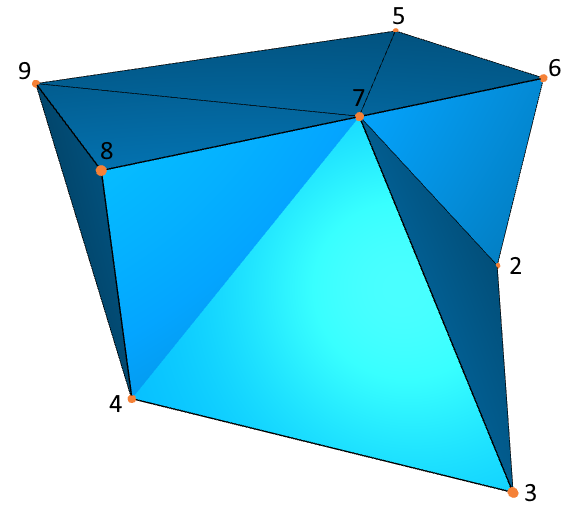
\includegraphics[width=0.25\textwidth]{images/versatile-front.png}
        \pause
        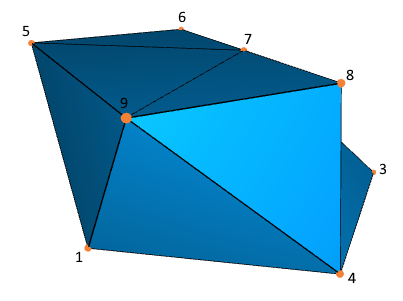
\includegraphics[width=0.3\textwidth]{images/versatile-back.png}
        \pause
        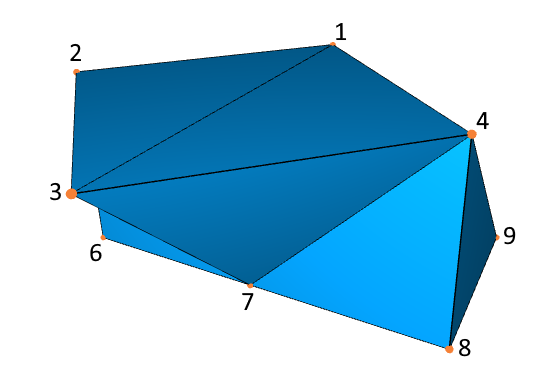
\includegraphics[width=0.33\textwidth]{images/versatile-square.png}
    \end{center}
\end{frame}

\begin{frame}{Isometries}
    \begin{definition}
        Let $n \in \N$, $V$ an euclidean $K$ vectorspace (with metric $d: V \times V \to K$).
        Then $\phi: V \to V$ is called an \emph{isometry} if \pause
        $$
            \forall x, y \in V : d(x, y) = d(\phi(x), \phi(y)).
        $$
    \end{definition}
    \pause
    \textbf{Note:} An isometry is always a combination of an affine transformation and an orthogonal matrix. Such an isometry $\phi = (A, a)$ operates as 
    $$
        (A, a)(x) \coloneqq A \cdot x + a.
    $$
    \pause
    The isometries of a given euclidean vectorspace are a group with the operation 
    $$
        \left( (A, a) \circ (B, b) \right) (x) \coloneqq (A \cdot B, A\cdot a + b)
    $$
    denoted by $E(n)$ \pause ($ \implies E(n) = O(n) \ltimes \R^n$).
\end{frame}
\begin{frame}{Wallpaper Groups}
    \begin{definition}{Crystallograhpic/Wallpaper Groups}
        Let $\Gamma \leq E(n)$ a subgroup of the group of isometries of dimension $n$.\\
        Then $\Gamma$ is called \emph{crystallographic group} if $\Gamma$ is cocompact and discrete, it is called \emph{wallpaper group} if $n=2$.
    \end{definition}
    \pause
    \begin{definition}
        Let $\Gamma \leq E(n)$. \\
        Then $\Gamma$ is cocompact if the space $E(n) / \Gamma$ is compact.
    \end{definition}
    \pause
    \begin{block}{Proposition (\cite[Prop. 1.9]{szczepanski2012geometry})}
        Let $\Gamma \leq E(n)$. \\
        Then $E(n)/\Gamma$ is compact iff the orbit space $\R^n / \Gamma$ is compact.
    \end{block}
\end{frame}

\begin{frame}{Examples of wallpaper groups}
    \vspace{-3em}
    \begin{alignat*}{2}
    \action<+->{
    &p1 \coloneqq \\
    &\left< 
        \left( \begin{pmatrix} 1 &0 \\ 0 &1\end{pmatrix}, \begin{pmatrix} 1 \\ -1 \end{pmatrix}\right), 
        \left( \begin{pmatrix} 1 &0 \\ 0 &1\end{pmatrix}, \begin{pmatrix} 1 \\ 1 \end{pmatrix}\right) \right> \\ }
    \action<+->{
    &pg \coloneqq \\
    &\left< 
        \left( \begin{pmatrix} 0 &-1 \\ -1 &0\end{pmatrix}, \begin{pmatrix} 2 \\ 0 \end{pmatrix}\right), 
        \left( \begin{pmatrix} 1 &0 \\ 0 &1\end{pmatrix}, \begin{pmatrix} 1 \\ 1 \end{pmatrix}\right) \right> \\ }
    \action<+->{
    &p4 \coloneqq \\
    &\left< 
        \left( \begin{pmatrix} 0 &1 \\ -1 &0\end{pmatrix}, \begin{pmatrix} 0 \\ 2 \end{pmatrix}\right), 
        \left( \begin{pmatrix} 0 &-1 \\ 1 &0\end{pmatrix}, \begin{pmatrix} 0 \\ -2 \end{pmatrix}\right),\left( \begin{pmatrix} -1 &0 \\ 0 &-1\end{pmatrix}, \begin{pmatrix} 0 \\ 0 \end{pmatrix}\right) \right>}
    \end{alignat*}
\end{frame}

\begin{frame}{Planar Assemblies of the Versatile Block}

\end{frame}

\section{Mechanics and Simulation}
\begin{frame}{Finite Element Method}
    
\end{frame}

\begin{frame}{Problem formulation}

\end{frame}

\begin{frame}{Simulation Setup}
    
\end{frame}

\subsection{Simulation Results}
\begin{frame}{Stresses}
    
\end{frame}

\section{Interlocking Flows}
\begin{frame}{Combinatorial Method}
    
\end{frame}

\begin{frame}{Combinatorial Results}
    
\end{frame}

\section{Outlook}

\begin{frame}
    
\end{frame}

\appendix
\begin{frame}    
\printbibliography 
\end{frame}

\end{document}
